\section{Introduction}
All today's exercises are to be included in week 6 directory.
Open up composer playground by going to \url{https://composer-playground.mybluemix.net}.

\section{T4}
In the lecture we adapted the trader example available from hyperledger. From the hperledger composer-playground business network page, open up a new network with the following details:
\begin{itemize}
	\item name: t4
	\item namespace: org.t4.net
	\item Admin: admin@t4.net
\end{itemize}


Access the business network via the composer-playground interface and you should see a similar webpage as displayed in Fig \ref{fi:cp}. There are 4 files that we intend to control today; the first file contains some very basic information about the blockchain application you are building, please populate as appropriate.

\begin{figure}
	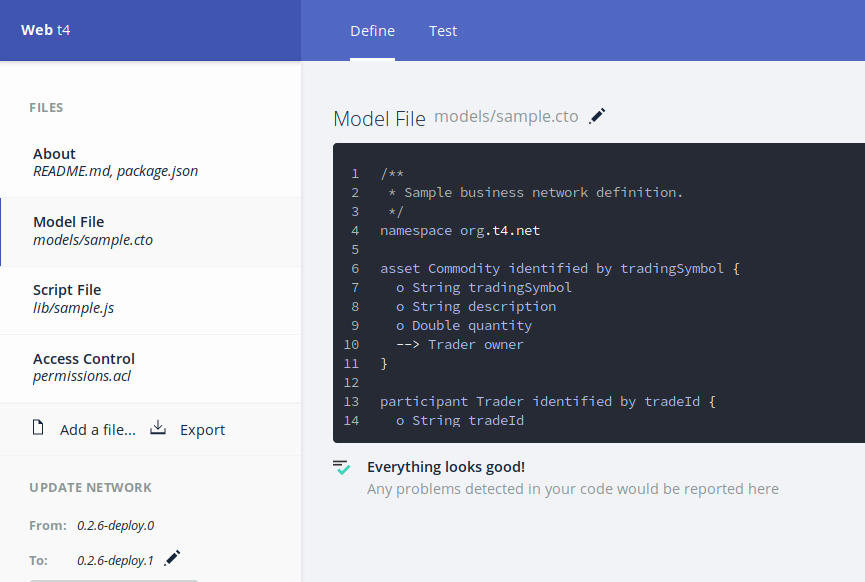
\includegraphics[scale=0.5]{cp}
\caption{Composer Playground development environment}
	\label{fi:cp}
\end{figure}

Complete the following instructions:
\begin{enumerate}
	\item Click on the Model File tab and enter the code in Fig \ref{fi:t4:cto} 
	\item Click on the Script File tab and enter the code in Fig \ref{fi:t4:js}
	\item Click on the Access Control tab and enter the code in Fig \ref{fi:t4:acl}
	\item Click deploy network and then Test
	\item Create two participants with id `0001' and `0002', respectively
	\item Create 1 commodity with id `0010' with ownership registered to trader with id, `0001'
	\item Complete the transaction that transfers the ownership of the commodity, `0010' to a new trader, `0002'. 
	\item Complete the transaction of the same resource, '0010', to a participant that does not exist. Does the transaction complete?
	\item Write the code using the method exist, prevent the above transaction from occuring and ensure that only existing participants can be the new owner.
\end{enumerate}

\begin{figure}
	\lstinputlisting[language=CTO]{t5/models/sample.cto}
	\caption{CTO code for t4 business network archive}
	\label{fi:t4:cto}
\end{figure}

\begin{figure}
	\lstinputlisting[language=JavaScript,lastline=12]{t5/lib/sample.js}
	\caption{JavaScript code for t4 business network archive}
	\label{fi:t4:js}
\end{figure}


\begin{figure}
	\lstinputlisting[language=ACL]{t5/permissions.acl}
	\caption{Access Control code for t4 business network archive}
	\label{fi:t4:acl}
\end{figure}


\section{Add Method}

In this section we are going to Add a new member of staff. Add the following code in Figs \ref{fi:t5:acl}, \ref{fi:t5:cto} and \ref{fi:t5:js} to your Access Control File, Model File and Script File in composer playground, respectively.

Complete the following:
\begin{itemize}
	\item Create three users, with clerk, consultant and manager status
	\item Issue new ID and wallets for these three users, call them clerk, consultant and manager
	\item Enter the system as a manager and test the addStaff function. Does it work? Look for console.log output.
	\item Enter the system as a clerk and test the addStaff function. Does it work? Look for the error.
	\item Complete your blockchain by introducing a new function that removes a member of staff from the participant registry, use the lecture notes and hyperledger website to help you.
	\item Test and evaluate your remove function, are there any restrictions and can they be overcome?
\end{itemize}

\begin{figure}
	\lstinputlisting[language=ACL]{t7/permissions.acl}
	\caption{Access Control code for allowing create privileges to add staff business network archive}
	\label{fi:t5:acl}
\end{figure}


\begin{figure}
	\lstinputlisting[language=CTO,lastline=11]{t7/models/sample.cto}
	\vdots
	\lstinputlisting[language=CTO,firstline=32,lastline=34,firstnumber=32]{t7/models/sample.cto}
	\caption{CTO code for adding Status to business network archive}
	\label{fi:t5:cto}
\end{figure}

\begin{figure}
	\lstinputlisting[language=JavaScript,firstline=27,firstnumber=27]{t7/lib/sample.js}
	\caption{JavaScript code for Adding member of staff to business network archive}
	\label{fi:t5:js}
\end{figure}


